\newpage
\section{Vector Space Retrieval Model: Basic Idea}

VSM - Vector Space Model

\subsection{Vector Space Model (VSM): Illustration}

\begin{figure}[H]
    \centering
    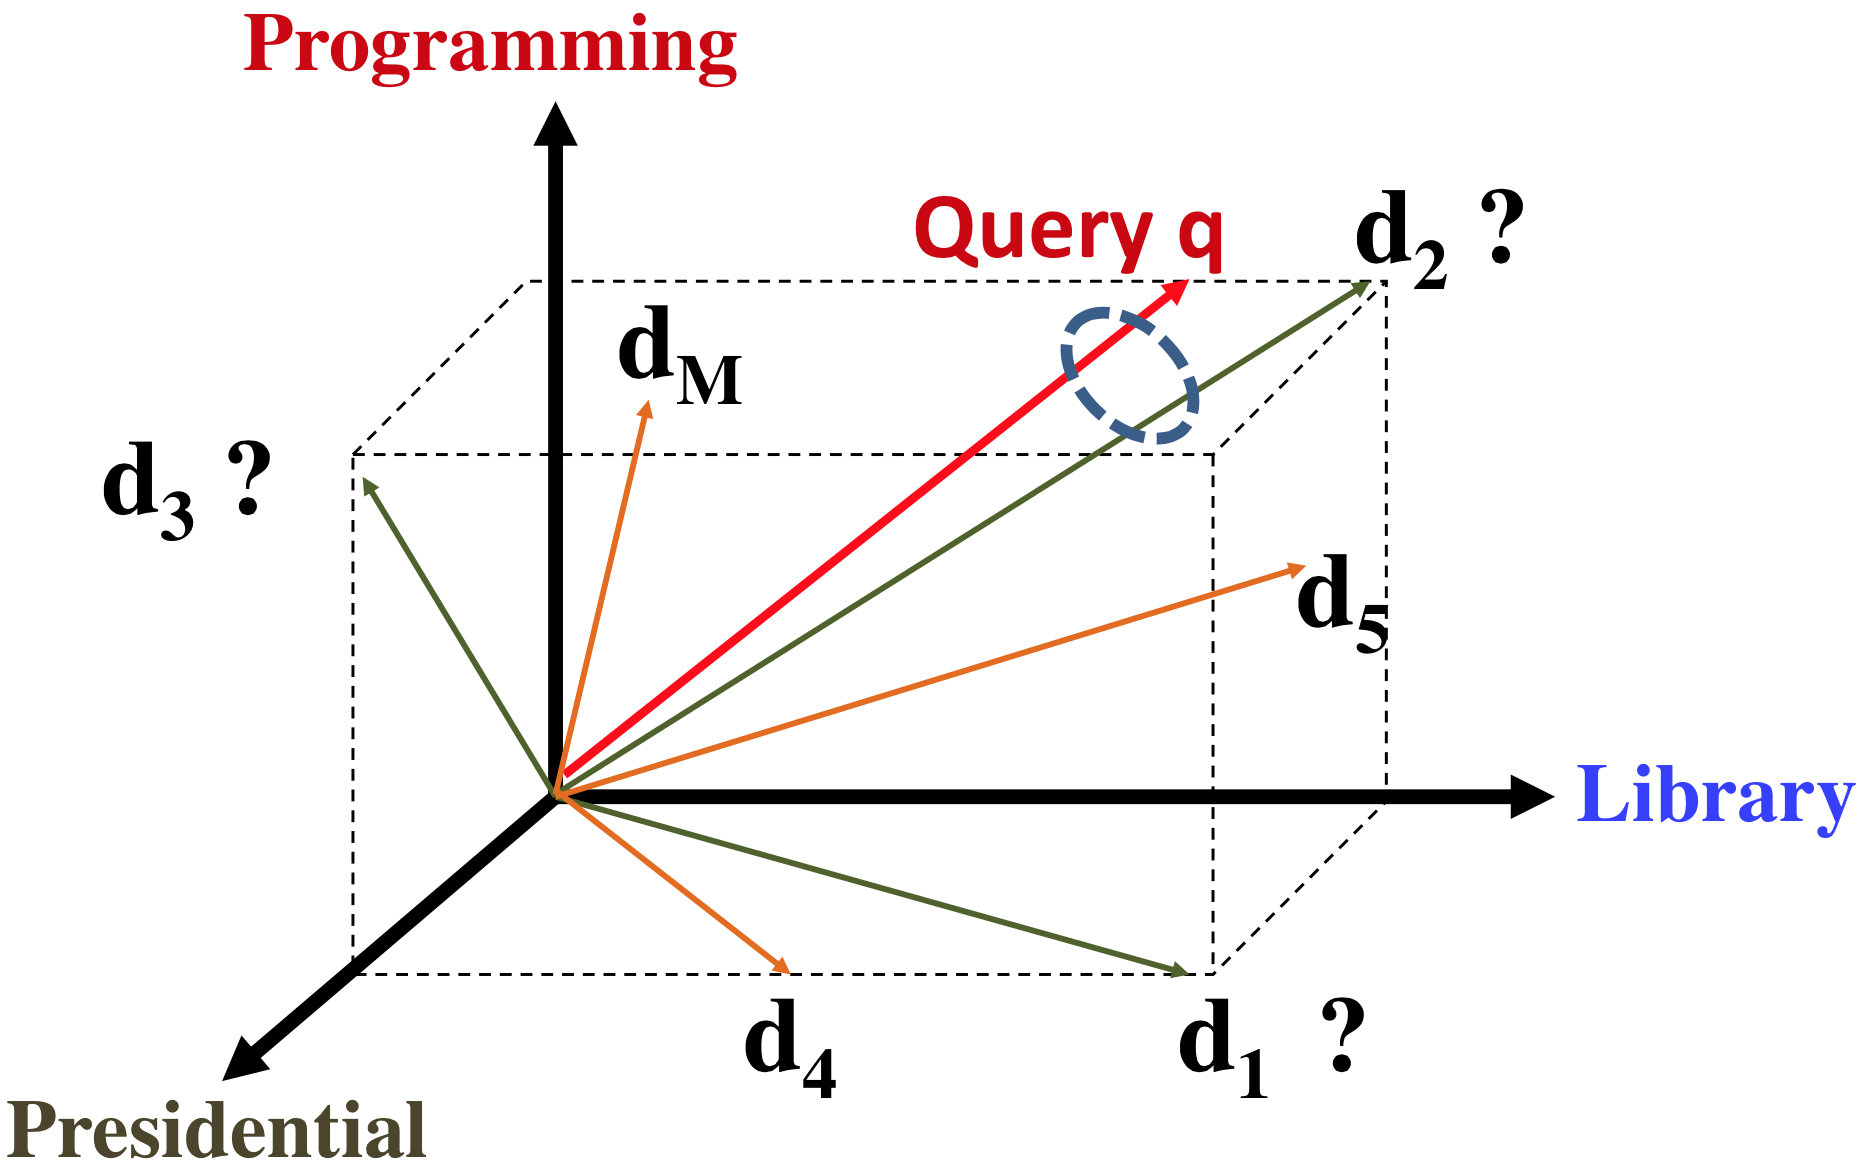
\includegraphics[width=\linewidth]{VSM.png}
\end{figure}


\subsection{VSM Is a Framework}
\begin{itemize}
\item Represent a doc/query by a term vector
\begin{itemize}
\item \textbf{Term}: basic concept, e.g., word or phrase
\item Each term defines one dimension
\item N terms define an \textbf{N-dimensional space}
\item \textbf{Query vector}: $q=(x_1, \dots x_N), x_i \in \Re$ is query term weight 
\item \textbf{Doc} vector: $d=(y_1, \dots y_N), y_j \in \Re$ is doc term weight
\end{itemize}
\item $relevance(q,d) \propto similarity(q,d)=f(q,d)$
\end{itemize}


\subsection{What VSM Doesn’t Say}
\begin{itemize}
\item How to define/select the “basic concept” – Concepts are assumed to be orthogonal
\item How to place docs and query in the space (= how to assign term weights)

\begin{itemize}
\item Term weight in query indicates importance of term 
\item Term weight in doc indicates how well the term characterizes the doc
\end{itemize}

\item How to define the similarity measure
\end{itemize}
